\section{Implementation}
\label{sec:implementation}

Web application development framework \textit{Django}~\cite{django}, Web API toolkit \textit{Django REST Framework} (DRF)~\cite{drf} and Python~\cite{python} library \textit{django-filter}~\cite{django-filter} are used to operate \boatvtwo.
PostgreSQL~\cite{psql} is used to provide a database for the server-side applications of the software.
During the implementation phase, decisions regarding models of the database have been directed towards the UI utilizing the API for database queries and searches.
The models reflect the \ud\ format of sentences and annotations are saved as fields of word lines.

The annotation page has most of the functionalities of \boatvone.
Entries are validated and errors are displayed on the annotation page for annotators to see invalid edits in real time, according to the \ud\ framework~\cite{UD-git} and the language provided.

Python library \textit{spa\textsc{C}y}~\cite{spacy} is used to provide linear dependency graphs.
Another JavaScript-based linear dependency graph~\cite{spyssalo} making use of \textit{brat}~\cite{brat-vis} is used to provide graphs as well.
An annotator's preference regarding this may vary, thus, giving them visualization options is important.

\begin{figure}[tbh]
    \centering
    \frame{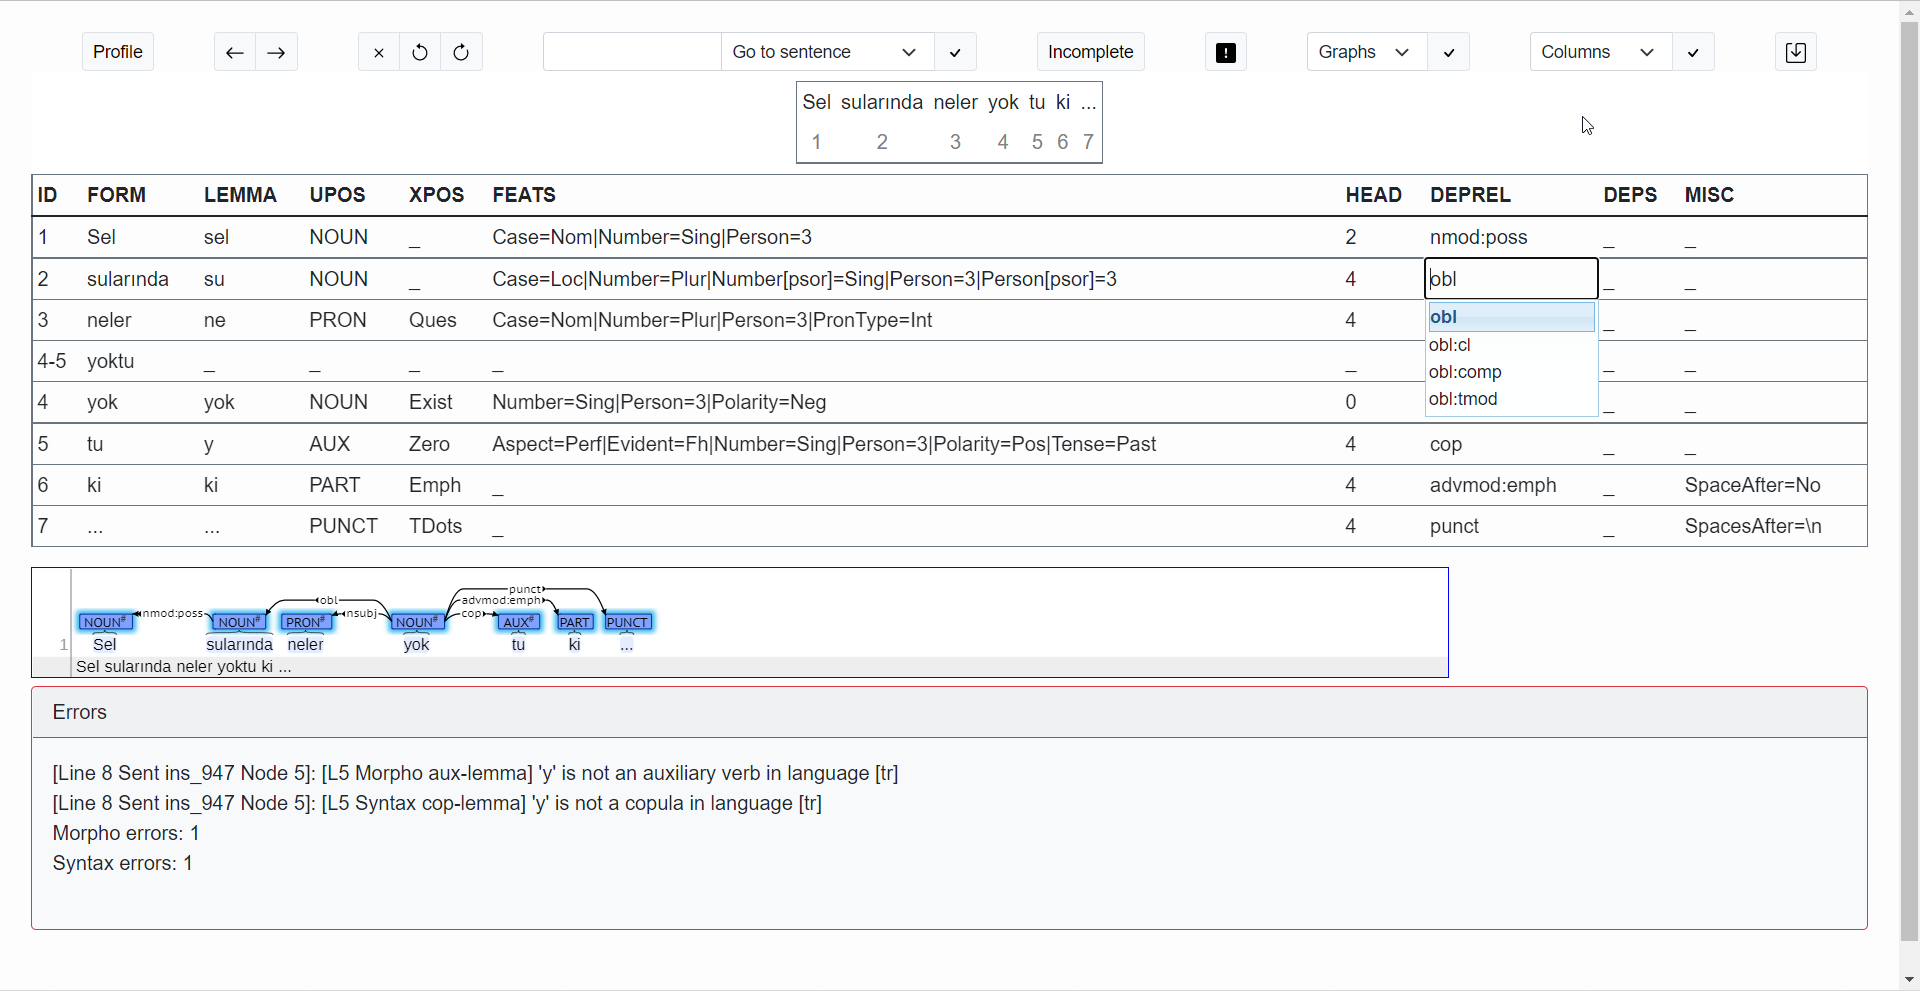
\includegraphics[width=1\textwidth]{figures/sample-annotation.png}}
    \caption{The annotation screen for the sentence ``Sel sularında neler yoktu ki...''.
        The annotator is choosing an annotation for the \deprel\ tag of the \form\ ``sularında''.
        The valid alternatives pop up based on the entry and can be selected via use of arrows. }
    \label{fig:anno-fig}
\end{figure}

\subsection{Features}
\label{sec:features}

There are many new features and improvements in this tool, as well as most of the functionality of \boatvone.

\begin{itemize}[before=\normalfont, font=\itshape, align=left]
    \item[Treebanks:]
        Multiple treebanks, with each one having its own sets of sentences, can be created in a single deployment.
        When uploading a \conllu\ file, a treebank is selected for the dataset in the file.

    \item[Loading files:]
        Instead of loading a dataset file before every annotation session, an annotator is able to upload a \conllu file for a treebank to the database for future use.
        The file is parsed and checked for its format. It's rejected if incorrectly formatted, otherwise uploaded to the database.
        This way, other annotators working with the same treebank don't have to provide the same file.

    \item[Annotation view:]
        The annotation page is very similar to the one on \boatvone~\cite{trk2020resources}, as seen in Figure~\ref{fig:anno-fig}.
        There is an annotation table for annotating fields in word lines of sentences.
        It also includes a dependency graph and an error card, both of which are in sync with the edits done on the table cells.
        Three different dependency graph representations are provided in this tool.
        Two of the graphs, which are both horizontal and linear, have been selected due to space considerations.
        The error card displays errors for the current annotation, validating it via the UD validation script.

    \item[Network-enabled search:]
        An important feature in this version is the ability to cross-check annotations by implementing a network for annotators where they can review the annotations done by other annotators.
        This can be helpful and a learning experience for annotators.

        For an actual example, the annotator, responsible for the \bountreebank's annotation, was annotating a sentence that had a Zodiac sign noun.
        Not being sure about how to annotate the noun's \upos\ tag, she searched the dataset in a text editor for similar sentences and encountered two different values with which nouns of Zodiac signs were annotated previously.
        Besides not helping how to choose a \upos\ tag, this raises a consistency issue within the treebank as well.
        One of the values was \noun\, the other one \propn.
        The annotator decided to use the one with more cases of annotation and proceeded to change the incorrect annotations based on their decision.
        This task could have been handled by a simple search of the database, rather than a manual search.
        We provide a search page and an API in this tool with which treebanks can be searched by \textit{sent\_id}s, \textit{text}s, all the UD tags and treebank names.
        With this, an annotator can easily make the treebank more consistent and reduce their frustration.

        Another example could be given by the various \textit{-ki} morphemes in Turkish.
        In the sentence ``Evdeki halılar yıkandı.'' (meaning \textit{The rugs at home were washed.}), the \textit{-ki} acts as an adjectivizer.
        In another sentence ``Benim halılarım yün, Ayşeninkiler sentetik.'' (meaning \textit{My rugs are woolen. Ayşe's are synthetic.}), it is pronominal.
        An annotator might not recall how a specific \textit{-ki} morpheme should be annotated, which can be remedied with a simple search.
        Annotators have informed us that such cases occur frequently when annotating MRLs.

        Also one other thing the inter-annotator agreement allows us to have is the possibility to see some anomalies in the Turkish part of the \ud\ framework.
        For example, if a sentence were annotated a way by many annotators but the \ud\ validation script were finding it invalid, this might indicate the validation were lacking in this respect of the Turkish language.
        Some modifications might be necessary and there could be a case for a proposal of change.

    \item[Annotation status:]
        We also provide a feature where an annotation has a status regarding its completeness.
        There are 3 different statuses and they are cycled through by the annotator in the annotation view.
        Status of an annotation is also shown in the search view, helping to select an appropriate case.
        Also there is another view where an annotator can list their completed, drafted or incomplete annotations, helping to keep track of what annotations have already been completed.

\end{itemize}
